\section{Merge Sort}
\label{sec:merge-sort-teo}

Desenvolvido por \href{https://en.wikipedia.org/wiki/John_von_Neumann}{Jon Von Neumann} em 1945, o \textit{Merge Sort} é um algoritmo de \href{https://en.wikipedia.org/wiki/Divide-and-conquer_algorithm}{dividir para conquistar}, que subdivide uma lista em singletons e os mescla em sublistas ordenadas até que exista apenas uma sublista, esta sublista é a lista original ordenada. Imagine o seguinte caso:

Você tem um baralho de cartas e gostaria de organizá-lo, seguindo o conceito do \textit{Merge Sort} você trabalha da seguinte forma:
\begin{itemize}
	\item \textbf{Divisão:} Primeiro você divide o baralho em dois baralhos menores. Cada um desses baralhos é dividido novamente até que cada sub-baralho tenha uma carta.
	\item \textbf{"Merge" (Mescla):} Nesse momento, com cada sub-baralho com uma carta, todos estão ordenados, então você começa a juntar os sub-baralhos comparando duas cartas de cada baralho e colocando-as em ordem crescente. Assim dois grupos de uma carta se tornam um baralho de duas cartas ordenadas. Em seguida, dois baralhos de duas cartas são mesclados para formar um baralho de quatro cartas, e assim por diante, até que todas as cartas estejam combinadas novamente, mas agora ordenadas.
\end{itemize}
\begin{figure}[!ht]
	\centering
	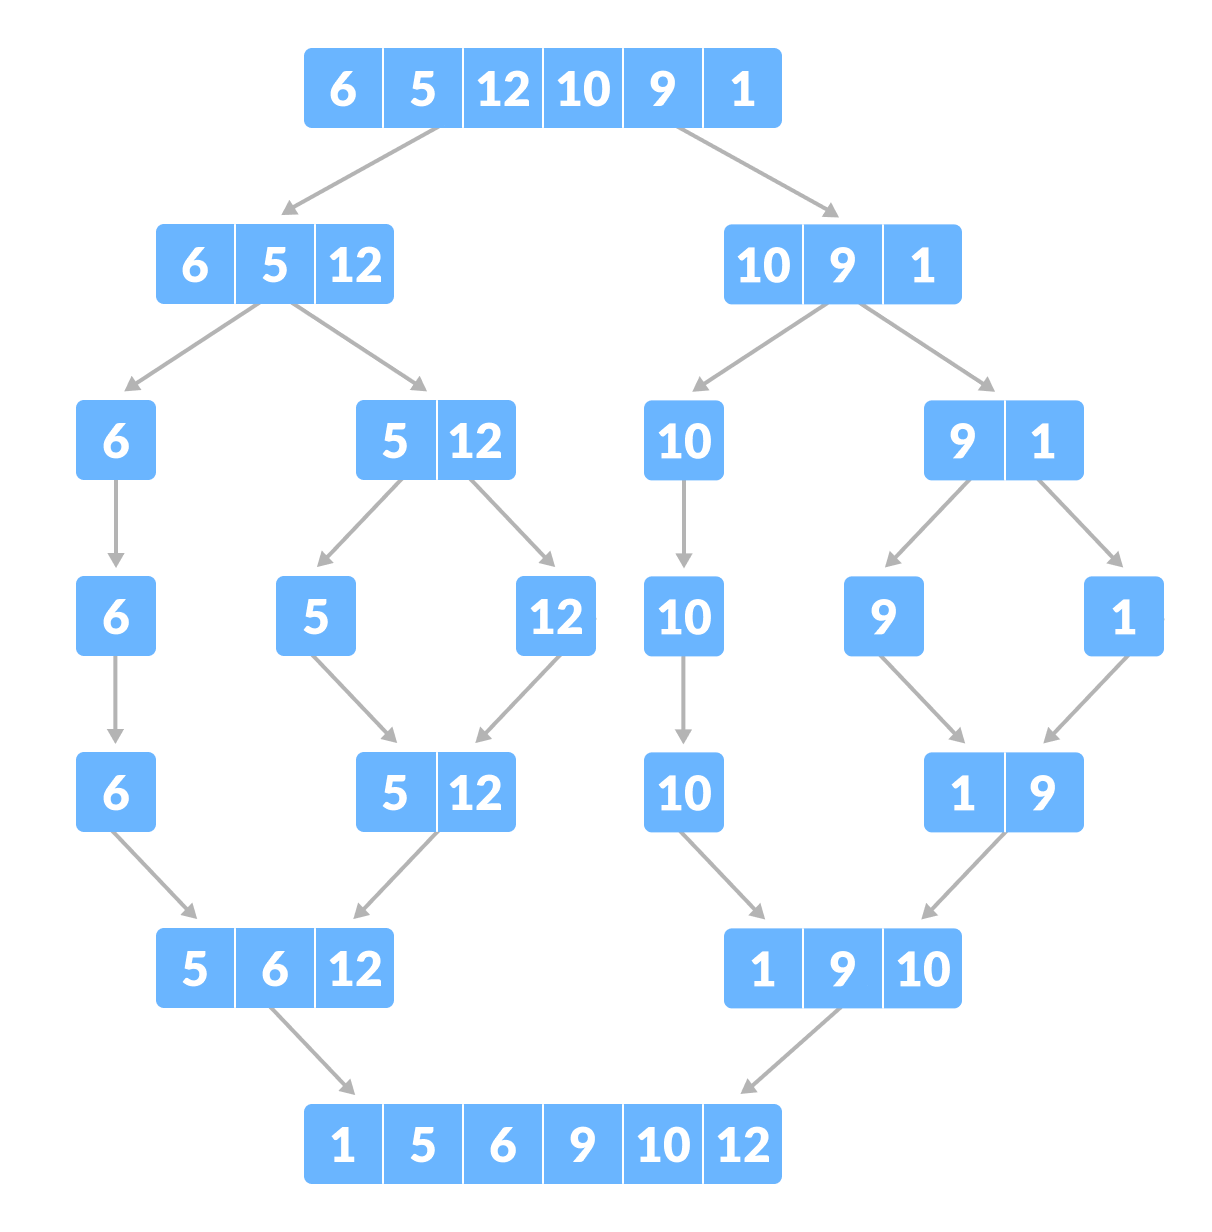
\includegraphics[scale=0.4]{figures/merge-sort-example_0.png}
	\caption{Diagrama exemplo de um Merge Sort}
	\label{fig:merge_sort_example_0}
\end{figure}

\FloatBarrier

\newpage

\subsection{Merge Sort Recursivo}

Dito isso, agora fica mais fácil estabelecer o pseudocódigo na forma recursiva. O caso base será se a lista tem no máximo um elemento, pois já está ordenada. No caso recursivo, pelo teorema da recursão temos acesso ao "caso anterior", ou seja a primeira metade e segunda metade da lista original ordenadas, portanto, podemos mesclá-las.

\begin{algorithm}
	\label{algo:merge_sort_pseudo}
	\begin{algorithmic}[1]
		\Require{$\mathbf{lista}  = x_0, x_1, \ldots, x_{N-1}$}
		\Function{MergeSort}{$\mathbf{lista}$}
		\If{tamanho da \textbf{lista} $\leq 1$} \Return
		\EndIf
		\State \Return {Merge(MergeSort($1^a$ metade da \textbf{lista}), MergeSort($2^a$ metade da \textbf{lista})}
		\EndFunction
	\end{algorithmic}
\end{algorithm}

\FloatBarrier

\subsection{Merge Sort Iterativo}

E em contraste com a abordagem anterior, a forma iterativa do Merge Sort se aproveita de estruturas de repetição aninhadas para que tenha acesso a índices específicos. E tais índices quando usados como argumento na função merge fazem com que a lista "quebrada" seja reconstruída de maneira ordenada. De forma que o loop mais externo controle a quebra da lista em sub-listas com a metade do tamanho anterior e o loop mais interno controla o índice inicial de cada sub-lista, conforme o pseudocódigo abaixo.

\begin{algorithm}
	\label{algo:merge_sort_it_pseudo}
	\begin{algorithmic}[1]
		\Require{$\mathbf{lista}  = x_0, x_1, \ldots, x_{N-1}$}
		\Function{MergeSortIt}{$\mathbf{lista}$}
		\State {tamanhoListas $\gets$ {$1$}}
		\Comment tamanho atual das sub-listas(variando de 1 até n/2)
		\State {índiceEsq $\gets$ {$1$}}
		\Comment index inicial da sub-lista à esquerda

		\For {tamanhoListas <= tamanho \textbf{lista} ; tamanhoListas $= 2$ $\cdot$ tamanhoListas}

		\For {índiceEsq $<$ tamanho \textbf{lista} $-$ $1$ ; índiceEsq $\cdot= 2$ $\cdot$ tamanhoListas}
		\State {meio $\gets$ índiceEsquerda $+$ tamanhoListas $-$ $1$}
		\State {fimDireita $\gets$ mínimo(índiceEsq $+$ $2$ $\cdot$ tamanhoListas, tamanho \textbf{lista} $-$ $1$)}
		\State {$merge$(lista, índiceEsq, meio, fimDireita)}
		\EndFor
		\EndFor
		\EndFunction
	\end{algorithmic}
\end{algorithm}

\subsection{Função auxiliar Merge}

\noindent
Nos resta agora apenas definir a função \textbf{Merge}, que vai ser responsável por mesclar duas listas que estão ordenadas. Para tal, a função deve comparar um elemento da primeira lista com um da segunda e anexar o menor elemento entre os dois no final da lista resultado. Por exemplo:

\begin{figure}[!ht]
	\centering
	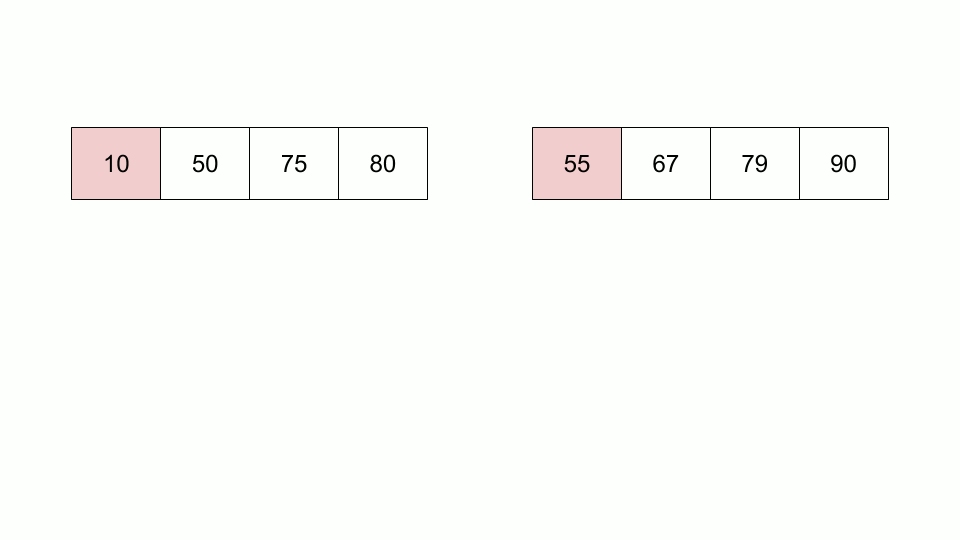
\includegraphics[scale=0.3]{figures/merge/merge-function-1.png}
	\caption{Comparando o primeiro elemento da primeira lista com o primeiro da segunda}
\end{figure}
\begin{figure}[!ht]
	\centering
	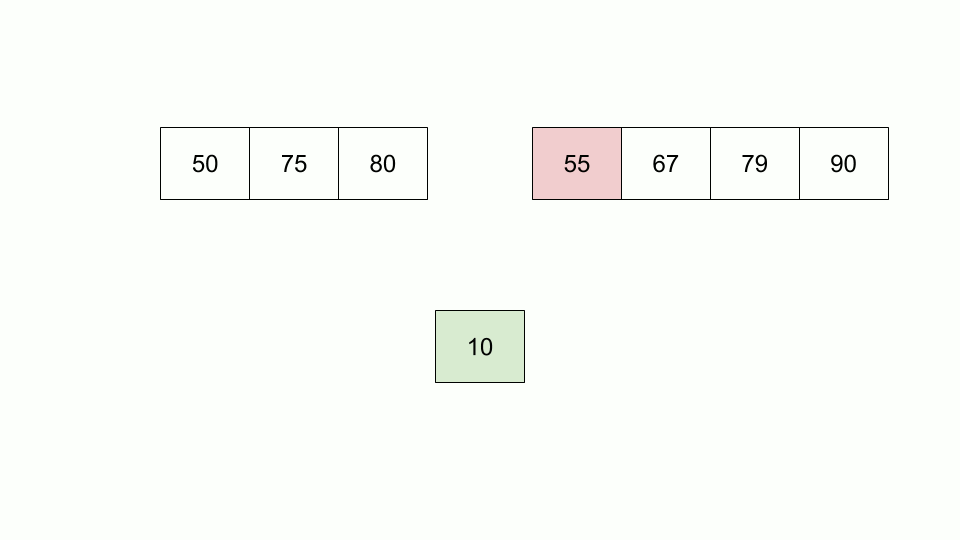
\includegraphics[scale=0.3]{figures/merge/merge-function-3.png}
	\caption{10 é menor que 55, então é anexado no final da lista resultado}
\end{figure}
\begin{figure}[!ht]
	\centering
	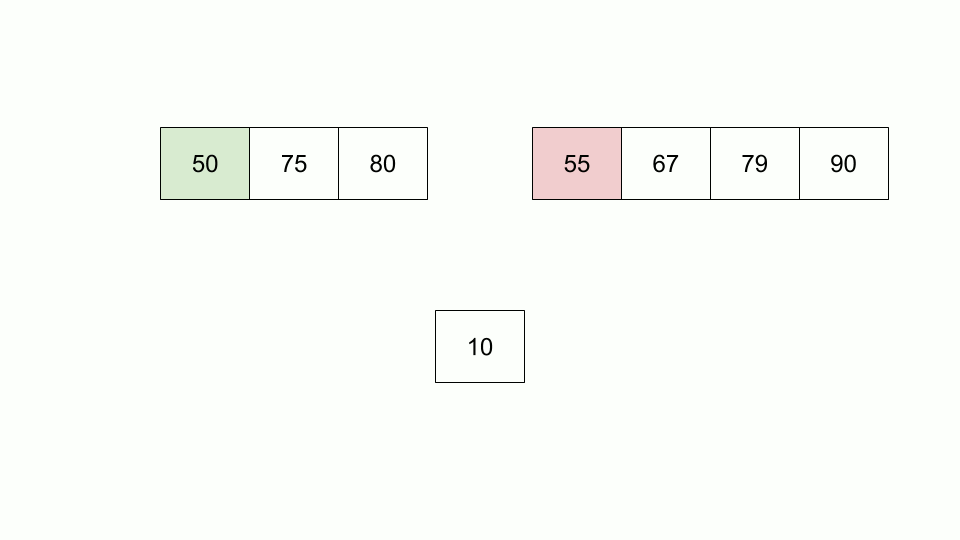
\includegraphics[scale=0.3]{figures/merge/merge-function-5.png}
	\caption{Comparando o próximo elemento da primeira lista}
\end{figure}
\begin{figure}[!ht]
	\centering
	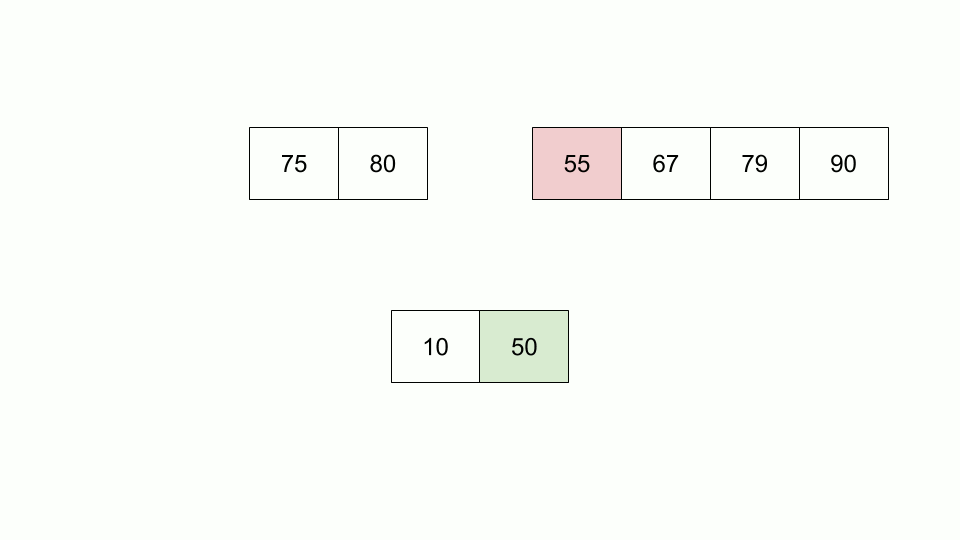
\includegraphics[scale=0.3]{figures/merge/merge-function-6.png}
	\caption{50 é menor que 55, então é anexado no final da lista resultado}
\end{figure}
\begin{figure}[!ht]
	\centering
	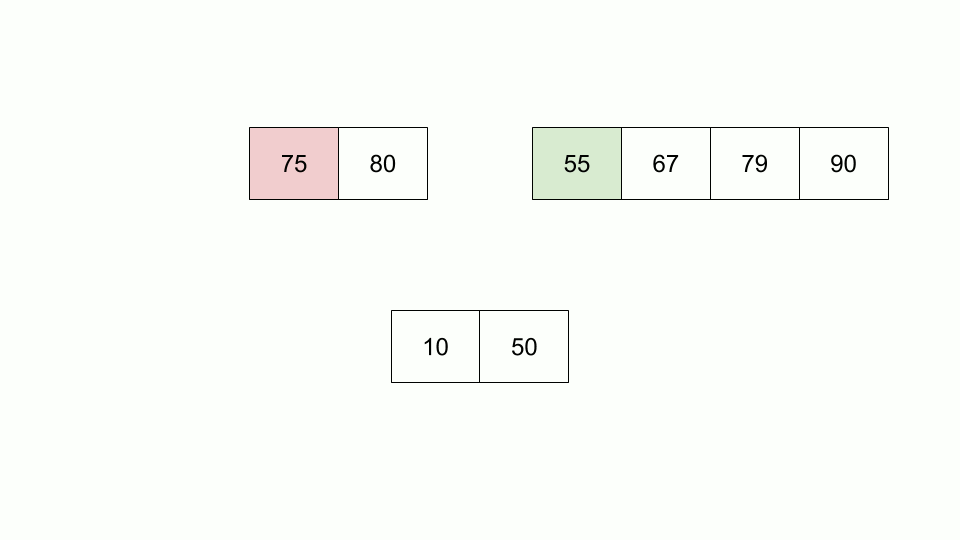
\includegraphics[scale=0.3]{figures/merge/merge-function-8.png}
	\caption{Comparando o próximo elemento da primeira lista}
\end{figure}
\begin{figure}[!ht]
	\centering
	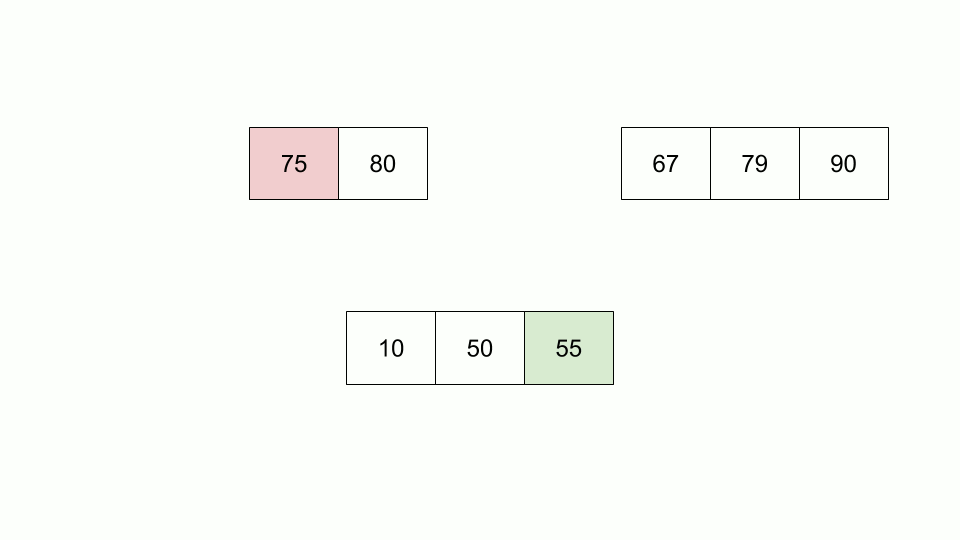
\includegraphics[scale=0.3]{figures/merge/merge-function-9.png}
	\caption{55 é menor, então é anexado no final da lista resultado}
\end{figure}
\begin{figure}[!ht]
	\centering
	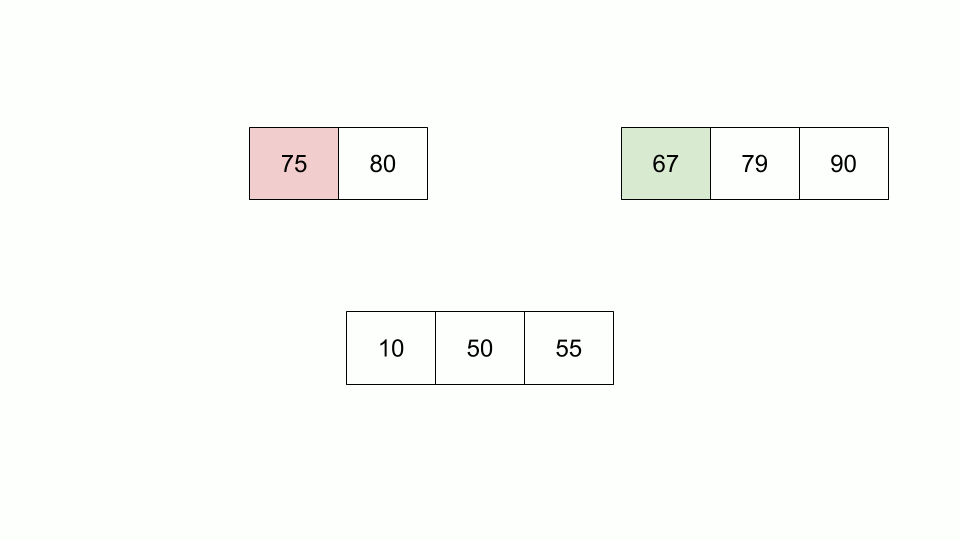
\includegraphics[scale=0.3]{figures/merge/merge-function-11.png}
	\caption{Comparando o próximo elemento da segunda lista}
\end{figure}

\FloatBarrier

E o algoritmo vai continuar até que a lista resultado esteja completa com os elementos da primeira e segunda lista.

Dito isso, construímos o pseudocódigo dessa função da seguinte forma:

\begin{algorithm}
	\label{algo:merge_aux_pseudo}
	\begin{algorithmic}[1]
		\Require{$\mathbf{listaEsquerda} = x_0, x_1, \ldots, x_{N - 1}$, $\mathbf{listaDireita} = y_0, y_1, \ldots, y_{M - 1}$}
		\Ensure{A \textbf{listaResultado} ordenada com os elementos da \textbf{listaEsquerda} e \textbf{listaDireita}}
		\Statex
		\Function{Merge}{$\mathbf{listaEsquerda}$, $\mathbf{listaDireita}$}
		\State $E, D, R \gets 0$ \Comment Esses serão os indexadores de cada lista
		\State $\mathbf{listaResultado} = 0, 0,\ldots, 0$
		\While{$E < N$ e $D < M$}
		\If{\textbf{listaEsquerda}(E) < \textbf{listaDireita}(D)}
		\State $\mathbf{listaResultado}(R).push(\mathbf{listaDireita}(D)$)
		\State $E \gets E + 1$ \Comment Partimos para o próximo elemento
		\Else
		\State $\mathbf{listaResultado}(R).push(\mathbf{listaEsquerda}(D)$)
		\State $D \gets D + 1$
		\EndIf
		\State $R \gets R + 1$
		\EndWhile
		\State $\rhd \text{ Como uma das listas vai esgotar primeiro que a outra, copiamos os elementos}$
		\State $\text{restantes para a }\mathbf{listaResultado}$
		\While {\textbf{listaEsquerda} ou \textbf{listaDireita} tiver elementos}
		\State adicione os elementos na \textbf{listaResultado}
		\EndWhile
		\State \Return \textbf{listaResultado}
		\EndFunction
	\end{algorithmic}
\end{algorithm}

\subsection{Análise de complexidade}
\label{anal:merge_sort}

Para analisar qual é a complexidade de tempo da \textbf{Merge sort}, nas suas duas versões, vamos estabelecer primeiro qual é a complexidade da função \textbf{Merge}. A partir do \href{algo:merge_aux_pseudo}{pseudocódigo} da função, é facil de ver que durante sua execução ela sempre vai percorrer o tamanho máximo entre a \textbf{listaEsquerda} e \textbf{listaDireita}, portanto, sua complexidade na notação de complexidade assintótica é $O(n)$, $\Theta(n)$ e $\Omega(n)$ para um tamanho de lista $n$.

\subsubsection{Análise da versão iterativa}

Observando a estrutura do \href{algo:merge_sort_it_pseudo}{pseudocódigo} dessa versão é possível perceber que ela é estritamente dependente do aninhamento de loops, e nada mais. E simplificando o algoritmo podemos observá-lo da seguinte maneira:

\begin{algorithm}
	\begin{algorithmic}[0]
		\For{$i \gets 1 ; i \leq n - 1 ; i = i \cdot 2$}
		\For{$j \gets 0 ; j < n - 1 ; j += i \cdot 2$}

		\State {$Merge()$}
		\EndFor
		\EndFor
	\end{algorithmic}
\end{algorithm}

Além disso, a versão iterativa usa uma abordagem inversa em relação à recursiva, isso pois a manipulação de índices faz com que a lista já comece "quebrada", faltando apenas ordenar as pequenas sub-listas entre si e mesclá-las. Sendo assim, apesar dos processos ocorrerem simultaneamente, podemos separar análise de complexidade da versão iterativa em duas partes: Reconstrução em sub-listas maiores e mesclagem ordenada das sub-listas.\\
Uma vez a lista começando completamente "quebrada", ou seja, com \textbf{n} sub-listas unitárias, o primeiro passo é transformá-las em \textbf{$\frac{n}{2}$} pares, e em seguida em \textbf{$\frac{n}{4}$} quartetos, até virarem uma única lista de tamanho \textbf{n}.

\begin{align*}
  T(n) = O(\log_2{n})
\end{align*}

Quebradas as sub-listas, como no primeiro loop as listas são unitárias, a ordenação acontece apenas em relação ao seu vizinho, formando pares. No segundo loop, a formação de quartetos implica na função merge ter que percorrer dois pares vizinhos a fim de achar o menor elemento, depois o par e a lista unitária a fim de achar o segundo menor, e é repetindo esse processo que a lista é mesclada em uma ordenada.

\begin{align*}
  T(n) = O(n)
\end{align*}

Analisadas as complexidades dos dois processos, como a mescla vai acontecer de acordo com quantas reconstruções da lista forem necessárias. Batas multiplicar as complexidades individuais para obter a complexidade total do algoritmo.

\begin{align*}
  T(n) & = O(n) \cdot O(\log_2{n})\\ 
       & = O(n \cdot \log_2{n})
\end{align*}

Analisado da perspectiva do pior caso, perceba que mesmo se tratando de uma lista já ordenada ainda sim será necessário quebrá-la e reconstruí-la tal qual uma desordenada. Sendo assim temos que a complexidade entre os cenários terá mesma ordem independente do quão perto ele seja o resultado final, ou seja, $O(n \cdot \log_2{n})$, $\Omega(n \cdot \log_2{n})$, $\Theta(n \cdot \log_2{n})$.

\subsubsection{Análise da versão recursiva}

Analisando o corpo da função, teremos dois casos: caso o tamanho da lista ($n$) seja menor ou igual 1 e caso contrário.

\begin{algorithm}
	\begin{algorithmic}[0]
		\If{tamanho da \textbf{lista} $\leq 1$} \Return
		\EndIf
		\State \Return {Merge(MergeSort($1^a$ metade da \textbf{lista}), MergeSort($2^a$ metade da \textbf{lista})}
	\end{algorithmic}
\end{algorithm}
\FloatBarrier

No primeiro caso, é facil de ver que a complexidade da função para uma lista de qualquer tamanho é constante, ou seja, $O(1)$, $\Theta(1)$ e $\Omega(1)$. Caso contrário, observa-se que a função chama a si mesmo duas vezes, uma para cada metade da lista. Ademais, a função \textit{Merge}, com complexidade linear para qualquer entrada, é chamada em cada etapa recursiva. Portanto, estabelecemos a relação de recorrência da \textit{Merge sort} recursiva como:


\begin{align*}
	T(n) =
	\begin{cases}
		O(1),                   & \text{se $n \leq 1$}  \\
		2T(\frac{n}{2}) + O(n), & \text{caso contrário}
	\end{cases}
\end{align*}

Uma vez estabelecida a relação de recorrência, podemos analisar a complexidade da função pelos 4 métodos vistos no curso. Entretanto, antes de começar, note que a Merge sort se comporta da mesma maneira para todos os casos, o que facilita o nosso cálculo de complexidade a seguir pelo método da \textbf{Substituição}.

Primeiramente, queremos demonstrar $T(n) \geq n \cdot \log_2 n$, para encontrar a complexidade na notação $\Omega$, que será equivalente as outras. Por indução no $n$, teremos:

% TODO: Colocar num enumerate
\begin{itemize}
  \item Caso $n = 1$:
    \begin{adjustwidth}{1em}{}
      Temos que:
      \begin{align*}
        T(1) = 1 \text{ \& } n \cdot \log_2 1 = 0
      \end{align*}
      Logo $T(1) \geq n \cdot \log_2 1$.
    \end{adjustwidth}
  \item Caso $n = k + 1$, para algum $k \in \mathbb{N}$:
    \begin{adjustwidth}{1em}{}
      Suponha que $T(n) \geq n \cdot \log_2 n$ (hipótese de indução). Calculemos:
      \begin{align*}
        T(n + 1) &= 2T\left(\frac{n + 1}{2}\right) + O(n) \\
                 &\geq 2 \cdot \frac{n + 1}{2} \cdot \log_2 \left(\frac{n + 1}{2}\right) + O(n) && \text{(hipótese de indução e função crescente)}\\
                 &= (n + 1)(\log_2 (n + 1) - 1) + O(n) \\
                 &= (n + 1)\log_2 (n + 1)) - n + 1 + O(n) \\
                 &\geq (n + 1)\log_2 (n + 1)
      \end{align*}
      Dessa forma $T(n + 1) \geq (n + 1)\log_2 (n + 1)$.
    \end{adjustwidth}
\end{itemize}


Pelo método da \textbf{Iteração}, expandimos a recorrência até um padrão ser identificado:

\begin{align*}
  T(n) &=  2T\left(\frac{n}{2}\right) + n \\
       &= 4T\left(\frac{n}{2}\right) + 2n \\
       &= 8T\left(\frac{n}{2}\right) + 4n \\
       &\vdots \\
       &= 2^iT\left(\frac{n}{2^i}\right) + in \\
\end{align*}

Dessa forma, agora identificamos o caso base da relação a partir de:

\begin{align*}
  \frac{n}{2^i} = 1 &\Longrightarrow n = 2^i \\
                    &\Longrightarrow \log_2 n = i
\end{align*}

Substituímos, temos que:

\begin{align*}
                                                              &= n \cdot T(1) + n \cdot \log_2 n \\
                                                              &= n + n \cdot \log_2 n 
\end{align*}

Portanto, a complexidade do merge sort se mantém consistente com os outros métodos e é $n \cdot \log_2 n$ nas notações assintóticas.

Ademais, também vamos usar o método da \textbf{Árvore de recorrência} para verificar o mesmo resultado. Comecemos estabelecendo a árvore de recursão:


\[\begin{tikzcd}[sep=small]
		&&&& {T(n)} \\
		\\
		&& {T(\frac{n}{2})} &&&& {T(\frac{n}{2})} \\
		& {T(\frac{n}{4})} & {T(\frac{n}{4})} &&&& {T(\frac{n}{4})} & {T(\frac{n}{4})} \\
		{T(\frac{n}{8})} & {T(\frac{n}{8})} & {T(\frac{n}{8})} & {T(\frac{n}{8})} && {T(\frac{n}{8})} & {T(\frac{n}{8})} & {T(\frac{n}{8})} & {T(\frac{n}{8})} \\
		\vdots & \vdots & \vdots & \vdots & \vdots & \vdots & \vdots & \vdots & \vdots
		\arrow[from=1-5, to=3-3]
		\arrow[from=1-5, to=3-7]
		\arrow[from=3-3, to=4-2]
		\arrow[from=3-3, to=4-3]
		\arrow[from=3-7, to=4-7]
		\arrow[from=3-7, to=4-8]
		\arrow[from=4-2, to=5-1]
		\arrow[from=4-2, to=5-2]
		\arrow[from=4-3, to=5-3]
		\arrow[from=4-3, to=5-4]
		\arrow[from=4-7, to=5-6]
		\arrow[from=4-7, to=5-7]
		\arrow[from=4-8, to=5-8]
		\arrow[from=4-8, to=5-9]
	\end{tikzcd}\]
\FloatBarrier

Uma vez estabelecida a árvore de recorrência, podemos tabular o tamanho da entrada, seu custo por nó e quantidade de nós para cada nível da árvore:


\begin{table}[h!]
	\centering
	\begin{tabular}{lrrr}
		\toprule
		Nível da árvore & Tamanho da entrada & Custo por nó    & Quantidade de nós \\
		\midrule
		0               & $n$                & n               & $1 = 2^0$         \\
		1               & $\frac{n}{2^1}$    & $\frac{n}{2^1}$ & $2 = 2^1$         \\
		2               & $\frac{n}{2^2}$    & $\frac{n}{2^2}$ & $4 = 2^2$         \\
		3               & $\frac{n}{2^3}$    & $\frac{n}{2^3}$ & $8 = 2^3$         \\
		$\vdots$        & $\vdots$           & \vdots          & \vdots            \\
		i               & $\frac{n}{2^i}$    & $\frac{n}{2^i}$ & $2^i$             \\
		\bottomrule
	\end{tabular}
\end{table}
\FloatBarrier

Em seguida, para estabelecer o somatório que calcula a complexidade da função, precisamos identificar o valor de $i$ para quando $T(\frac{n}{2^i}) = T(1)$, assim, teremos:

\begin{align*}
	\frac{n}{2^i} = 1 & \Longrightarrow n = 2^i      \\
	                  & \Longrightarrow \log_2 n = i
\end{align*}

Dessa forma, a complexidade da função para $\Omega$, $\Theta$ e $O$ será dada pelo resultado do somatório:

\begin{align*}
	\sum_{i = 0}^{\log_2 n} \frac{n}{2^i} \cdot 2^i & = \sum_{i = 0}^{\log_2 n}n  \\
	                                                & = n\sum_{i = 0}^{\log_2 n}1 \\
	                                                & = n \cdot \log_2 n
\end{align*}


Pelo método do \textbf{Teorema mestre}, o mesmo resultado ocorre em ainda menos etapas. Pelo teorema, temos que estabelecendo a relação de recorrência nessa forma:

$$
	T(n) = aT\left(\frac{n}{b}\right) + \Theta\left(n^{k}\right)
$$

Para algum $a \geq 1$, $b \geq 1$, e $k \geq 0$. Vale que:

\begin{enumerate}
	\item Se $a \geq b^k$, então $T(n)$ é $\Theta(n^{\log_b a})$.
	\item Se $a = b^k$, então $T(n)$ é $\Theta(n^k \cdot \log_b a)$.
	\item Se $a < b^k$, então $T(n)$ é $\Theta(n^k)$.
\end{enumerate}

A partir da \href{recc:rec_merge_sort}{relação de recorrência estabelecida}, tome $a = 2$, $b = 2$ e $k = 1$. Como $b^k = 2 = a$, logo, $T(n) = \Theta(n \cdot \log_2 n)$. Como foi estabelecido que o pior caso, o melhor e caso médio iam ter a mesma complexidade, logo, a \textit{Merge sort} também tem as complexidades $O(n \cdot \log_2 n)$ e $\Omega(n \cdot \log_2 n)$.

